\label{chapter-3}

This chapter will give an introduction to how existing process models can be evaluated and optimized. First, it will show how process steps can be eliminated using \textit{value added analysis} as part of the \textit{six sigma} initiative. After that, this chapter will give an introduction to methods for measuring metrics like time and cost of processes defined as \gls{bpmn} models to better evaluate two alternative processes.
\section{Six Sigma and Value Added Analysis}
\subsection{Introduction to Six Sigma}
% Fundamentals and Handbook for process management
The first analyzation and optimization technique discussed in this chapter originates from the six sigma initiative. The name six sigma stands for the interval of $6\sigma$ in the normal distribution that indicates the aimed success rate of $99.99966\%$ of a process \cite{siha2008business}\cite{vivekananthamoorthy2011lean}. A representation of the statistical meaning can be seen in figure \ref{fig:six-sigma}. Apart from the goal to decrease the error rate, $6\sigma$ is also a methodology for systematically improving other aspects of process quality \cite{tennant2017six}.

\begin{figure}[H]
	\centering
	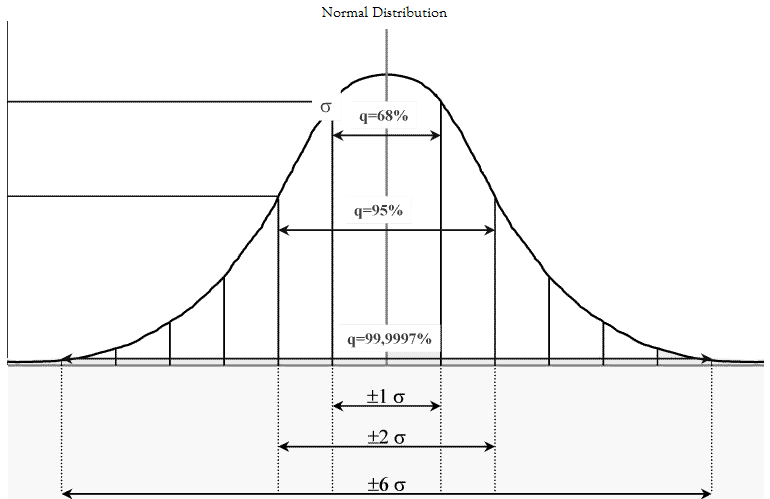
\includegraphics[width=0.7\columnwidth]{graphics/six-sigma}
	\caption{The standard normal distribution showing the $6\sigma$ interval (graphic from \cite{vivekananthamoorthy2011lean})} 
	\label{fig:six-sigma} 
\end{figure}

While countless tools are available as part of six sigma, the two main methodologies applied in these tools are \gls{DMAIC}, used for improving existing processes, and \gls{DMADV}, used when creating new processes \cite{selvi2014six}.

Applied in the context of (executable) business processes, six sigma provides a method to identify and eliminate inefficient or needless steps in a process, called \textit{value added analysis} \cite{vom2014handbook}. 


\subsection{Value Added Analysis (VAA)}\label{vaa}

The aim of the value added analysis is to determine the value of each activity in a process and identify activities that can be eliminated \cite{fundamentals}\cite{harrington2016value}. When performing value added analysis, every step in a process is classified by the kind of value it adds \cite{harrington2016value}: 

\begin{itemize}
	\item \textbf{RVA (Real value added)}: Activities that contribute to the external customers expected output are viewed as \textit{real value adding}. 
	\item \textbf{BVA (Business value added)}: Some activities in processes are not performed with the customer in mind but are needed to keep the company running. These are classified as \textit{business value adding}.
	\item \textbf{NVA (No value added)}: Activities that neither contribute to external customer requirements nor keep the business running are considered as \textit{non value adding}. There are two kinds of such steps, activities that are necessary because of bad process design (e.g. reworking, waiting, moving,...) and activities of bureaucratic nature (e.g. reporting, logging, ...).
\end{itemize}

To make this more practical, H. James Harrington provided a flowchart \ref{fig:VAA-flow} with which every activity can be classified into one of that three categories\cite {harrington2016value}.

\begin{figure}[H]
	\centering
	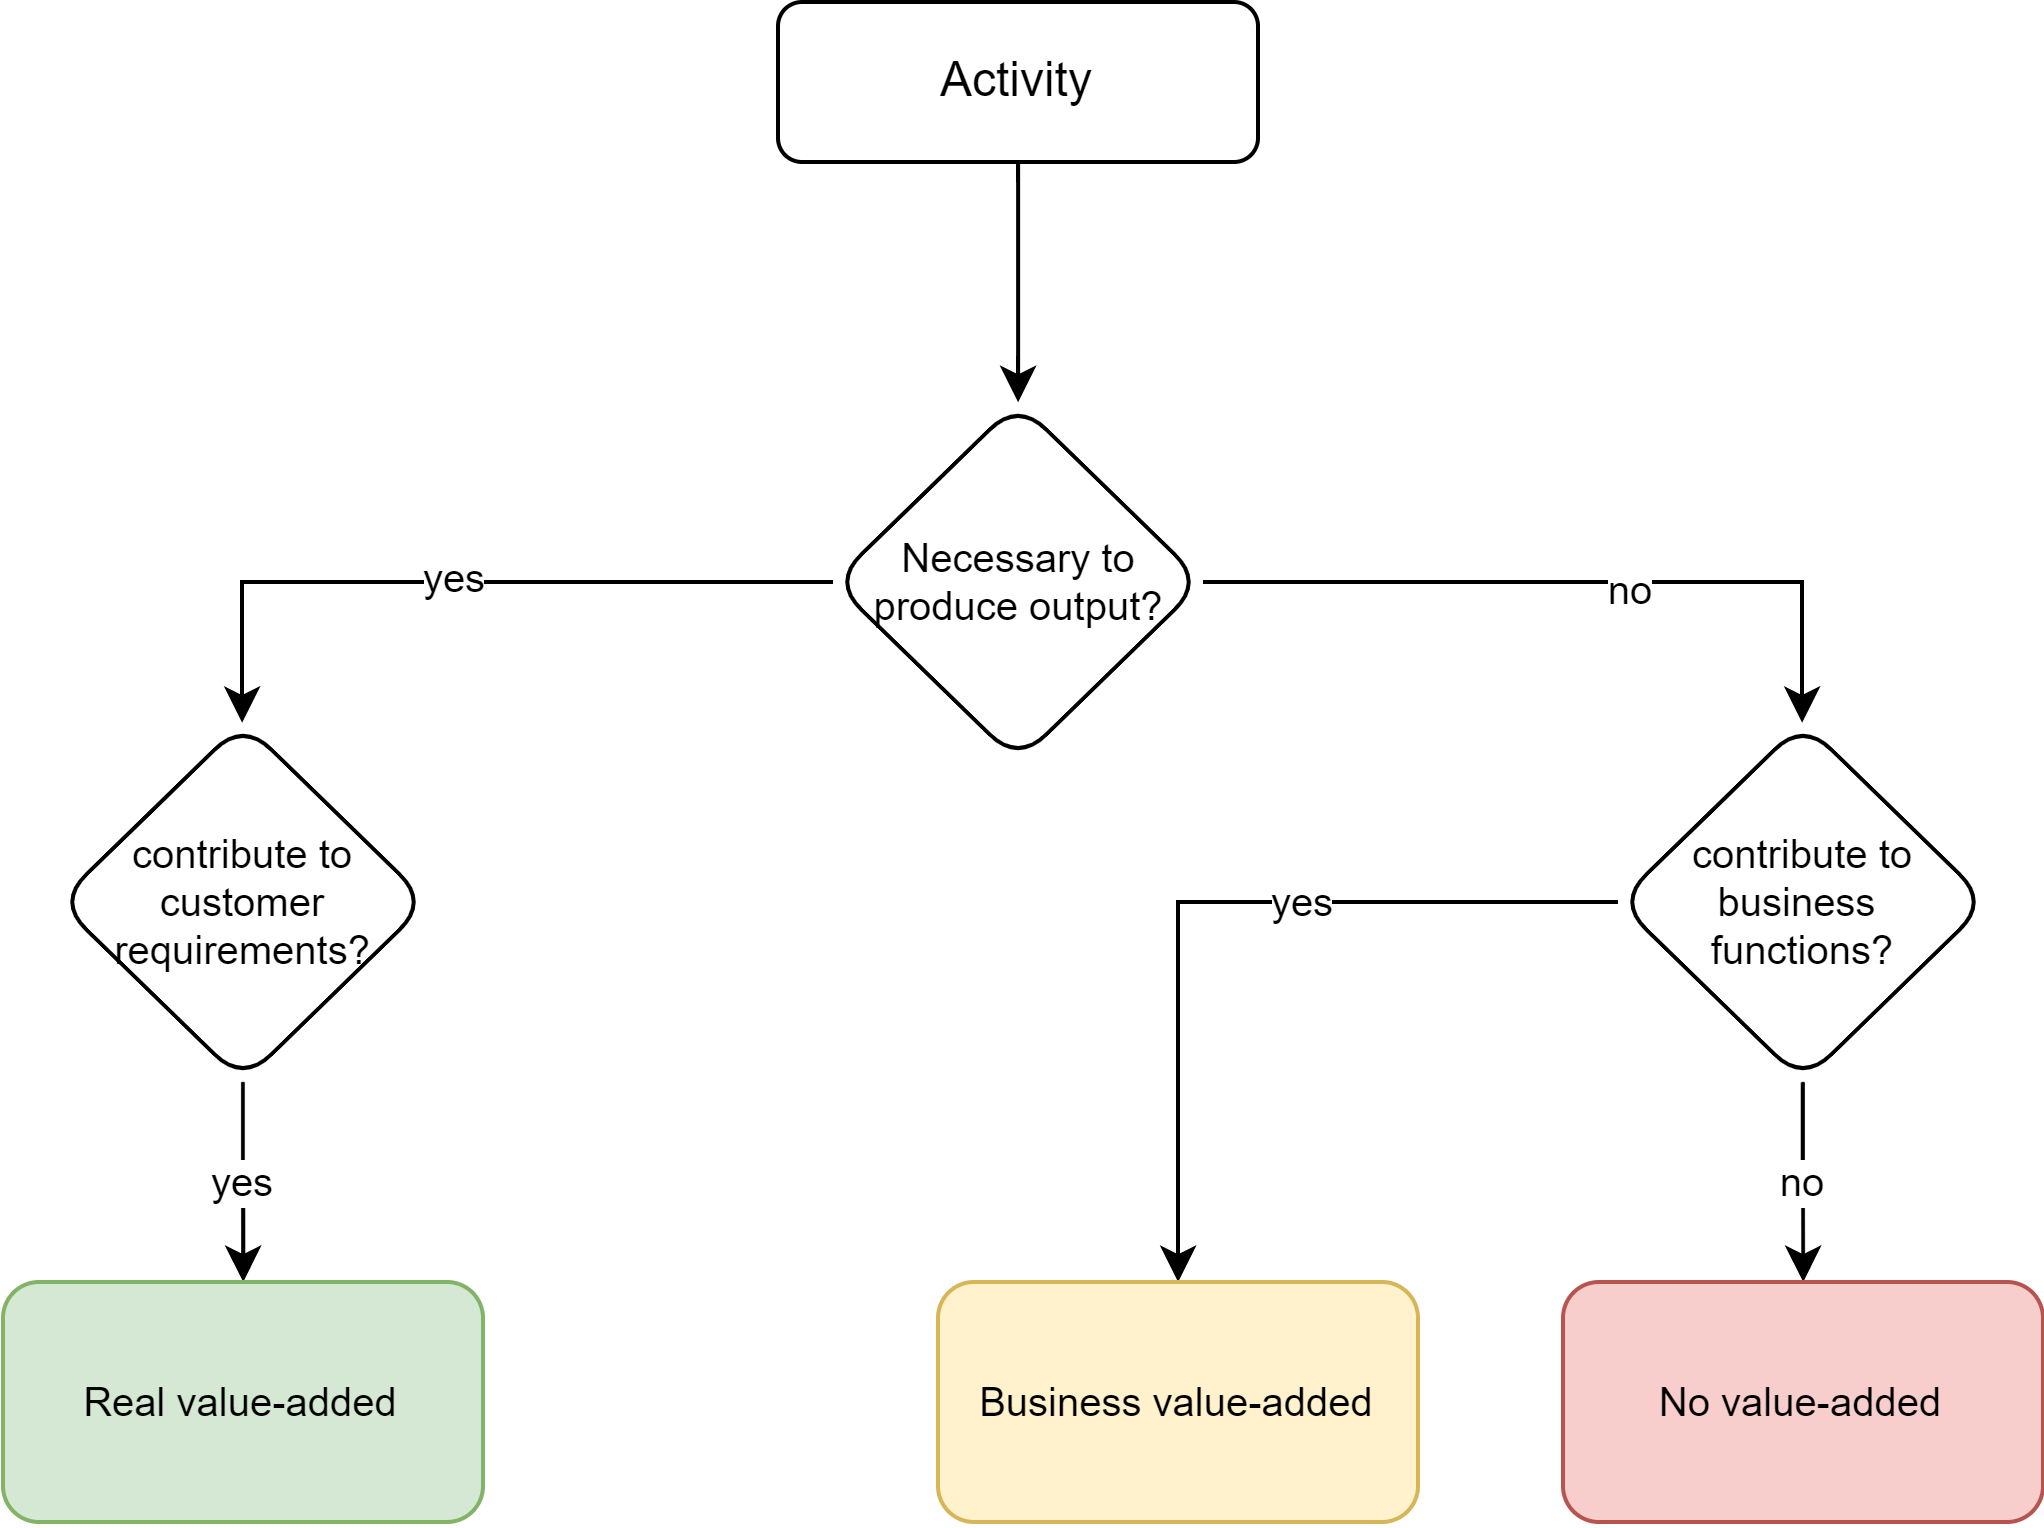
\includegraphics[width=0.8\columnwidth]{graphics/VAA}
	\caption{The value added analysis flowchart adapted from \cite{harrington2016value}} 
	\label{fig:VAA-flow} 
\end{figure}

To demonstrate the value added analysis, the exemplary \textit{Missing Part Process} will be used. This fictional process demonstrates what happens when a customer of a furniture shop reports a missing part in his/her order and requests a new part to be shipped. The corresponding process model is shown in figure \ref{fig:missing-part-process}

\begin{figure}[H]
	\centering
	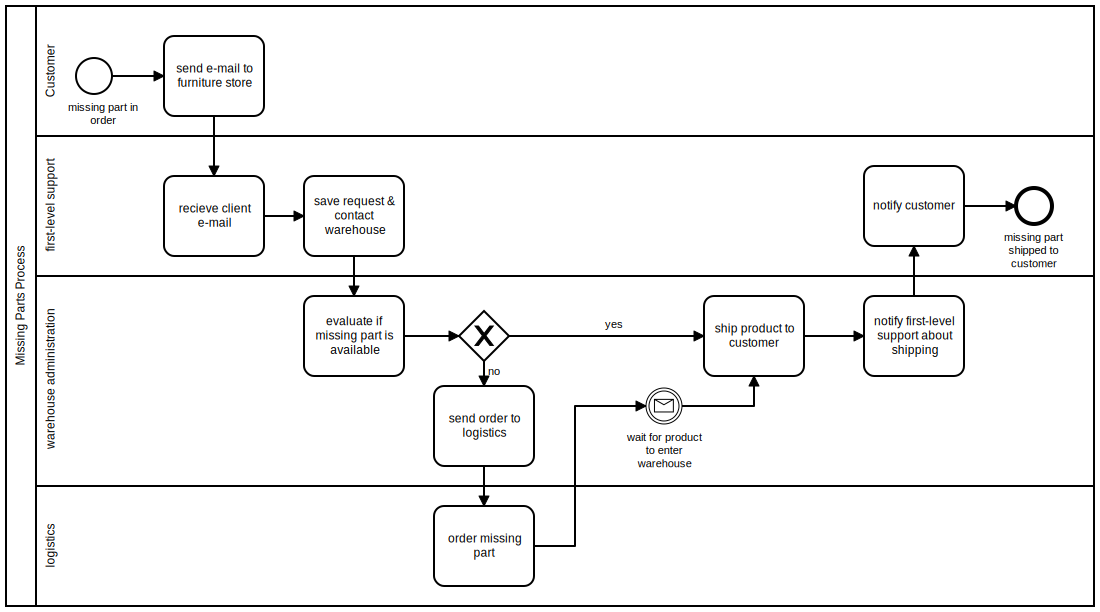
\includegraphics[width=1\columnwidth]{processes/missing-parts-process/missing-parts-process}
	\caption{The \textit{Missing Part Process} BPMN model} 
	\label{fig:missing-part-process} 
\end{figure}

In figure \ref{fig:VAA-missing-parts} the tasks in the missing parts process (figure \ref{fig:missing-part-process}) are colored according to their category after applying the flowchart in figure \ref{fig:VAA-flow}. Green tasks are real value adding activities, yellow tasks are business value adding activities and red tasks are no value adding activities. 

\begin{figure}[H]
	\centering
	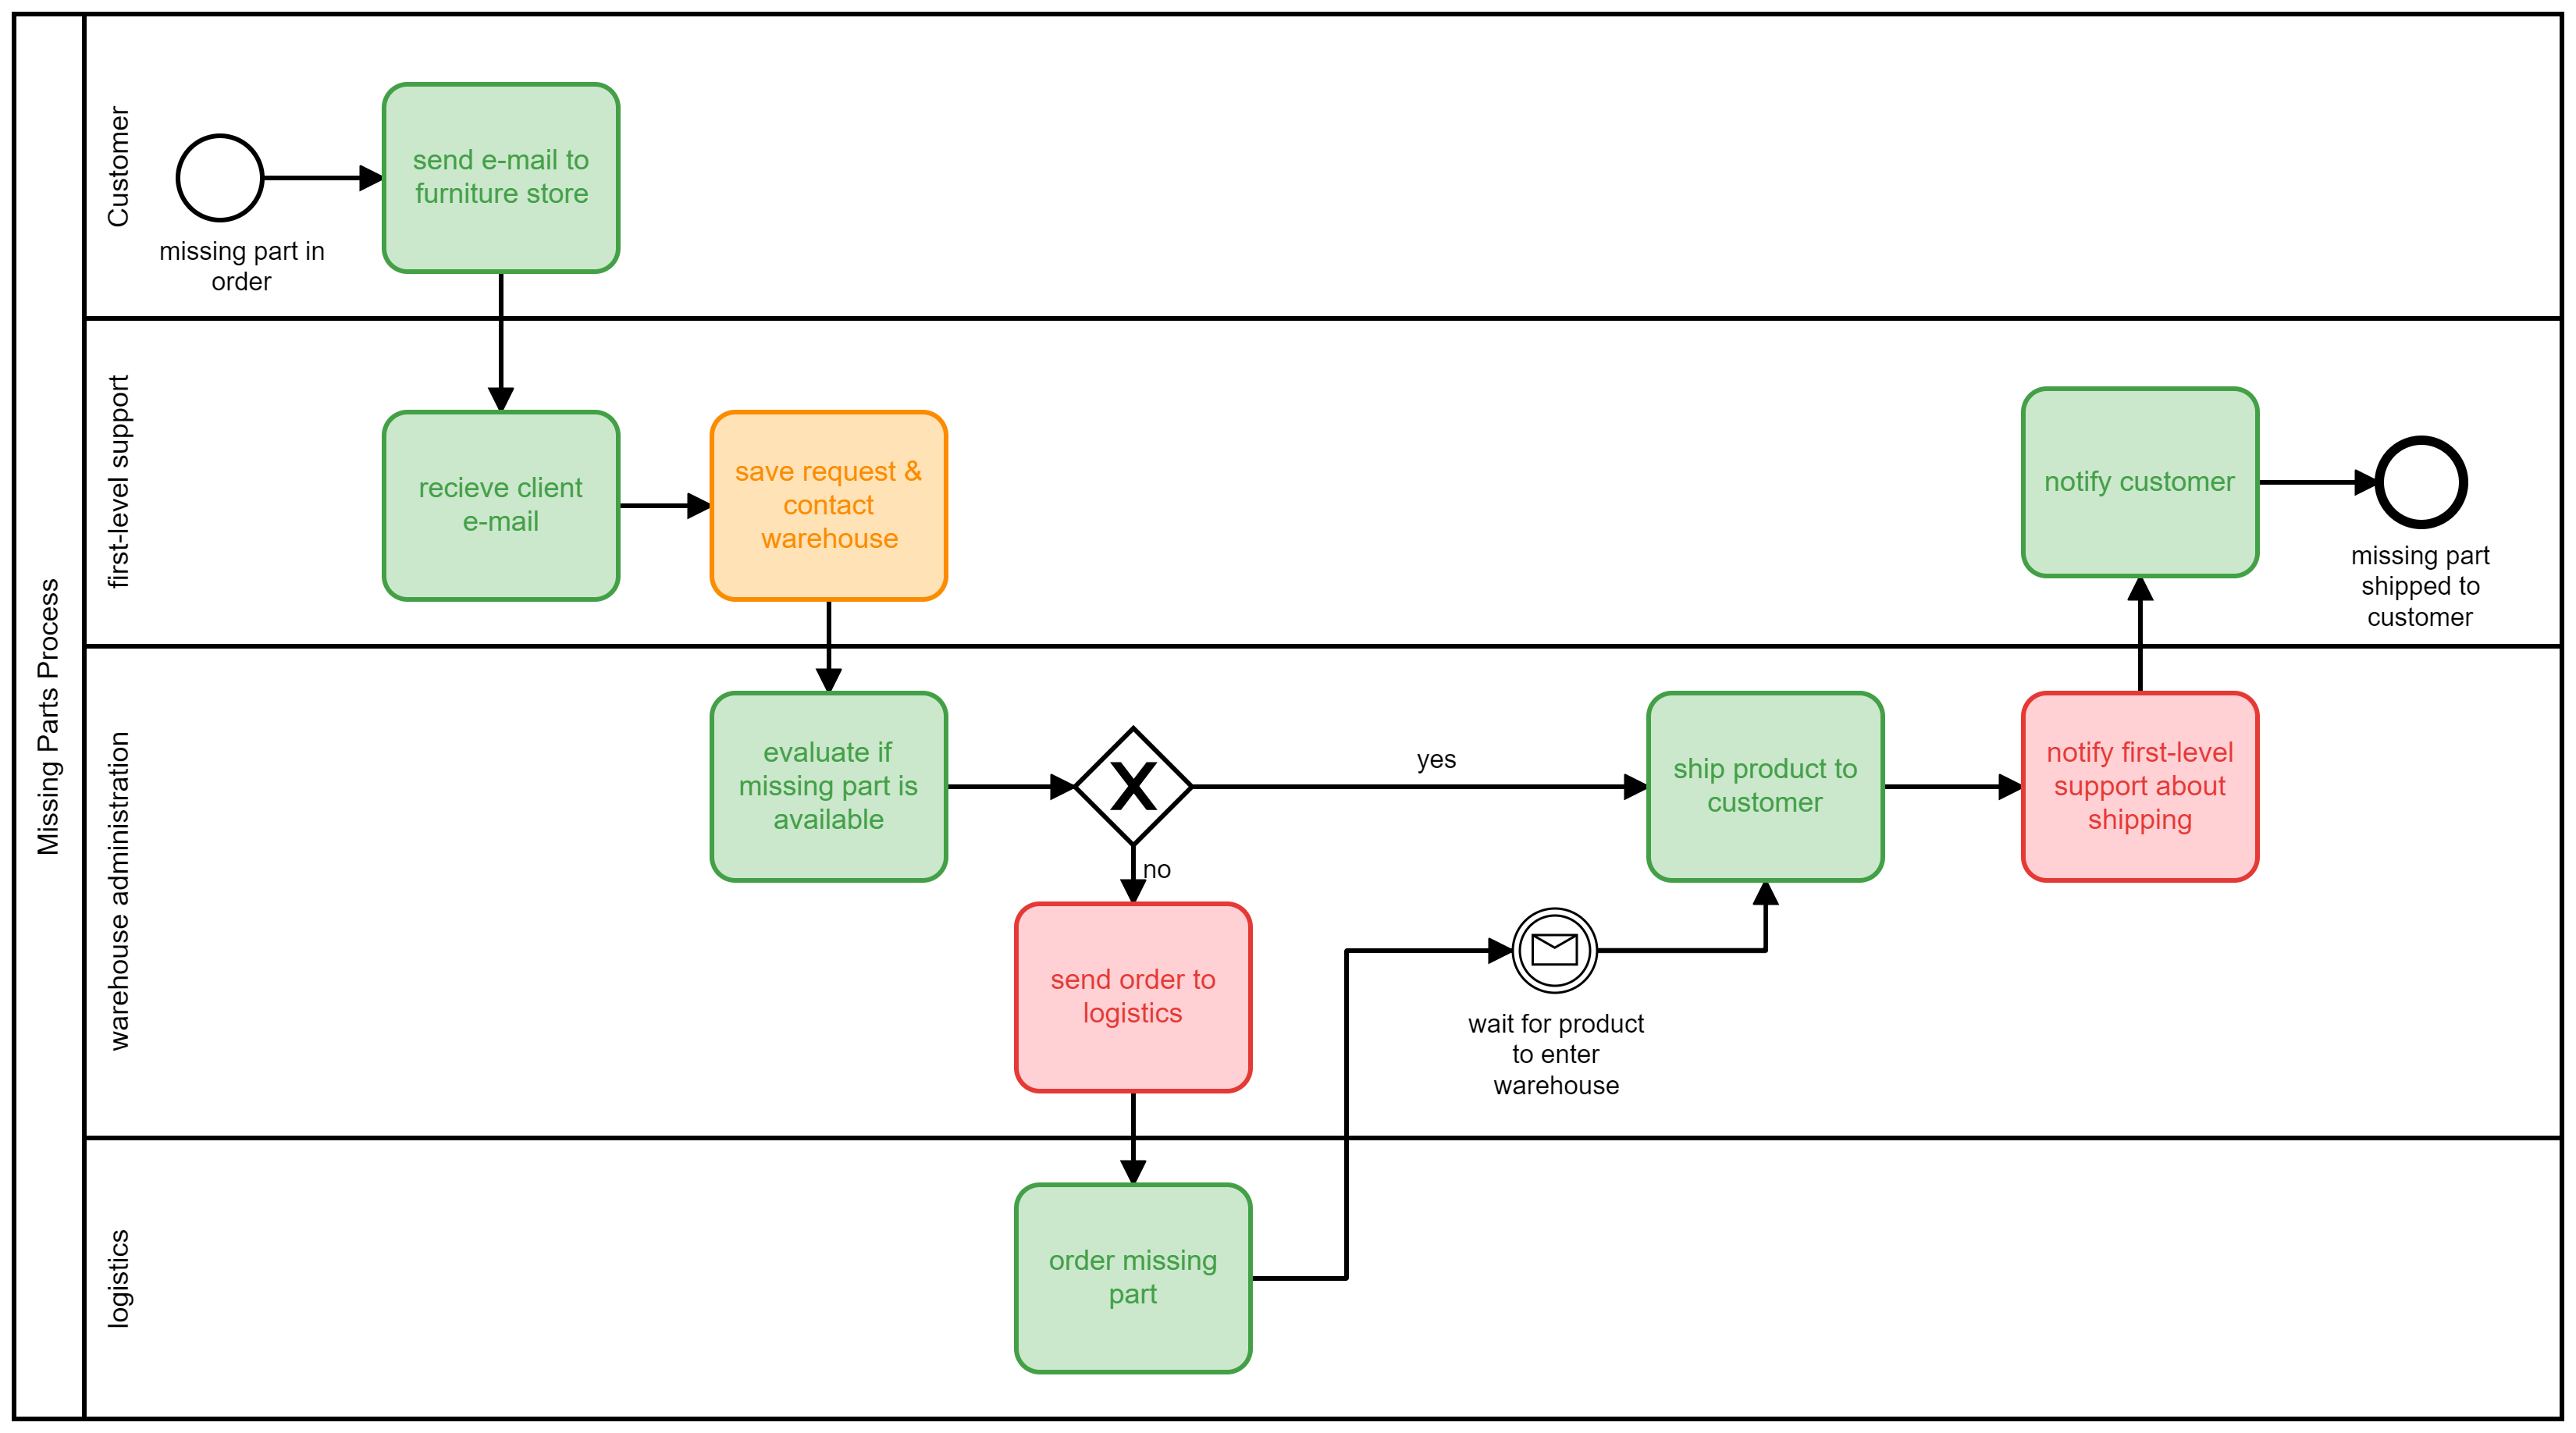
\includegraphics[width=1\columnwidth]{graphics/missing-parts-process-vaa}
	\caption{missing parts process (figure \ref{fig:missing-part-process}) with tasks colored based on their value} 
	\label{fig:VAA-missing-parts} 
\end{figure}

After this categorization is done, one can start with waste elimination. The first goal is to try to eliminate the impact of NVA activities. This can be done for example by automating the activity. In the context of the missing parts process (figure \ref{fig:missing-part-process}) this could mean automating the customer notification after the ordered product enters the warehouse. 

Another approach for waste elimination is minimizing handovers. For example, the process can be altered in a way, that the warehouse administration directly triggers the product ordering instead of sending the order to the logistics department. Apart from eliminating NVA steps, this is also the opportunity to evaluate BVA steps. If the BVA steps do not align with actual business goals or do not bring enough value to the business goal they are applied for, they should also be eliminated or simplified. \cite{fundamentals}\cite{harrington2016value}


\section{Quantitative Analysis}\label{quant}
To measure and justify changes in the status quo process, a quantitative method for analyzing and comparing alternative processes is needed. In the context of \gls{bpm}, accessible measures about three different dimensions of a process can be investigated: the process as a whole, resources involved in the process, and individual tasks in a process. \cite{fundamentals}

Before discussing methods for measuring process performance, it is necessary to define what is measured. The three key performance measures of a process are: cost, quality, and time\cite{fundamentals}

The following chapter will present methods for qualitative analysis of processes. Starting with the definition of the three dimensions of process performance. 

\subsection{Performance Measures}
As mentioned above, the performance of a process can be measured using the three dimensions:  cost, quality, and time. 
\paragraph{Cost}~\\
The purpose of process redesign is often to reduce cost or to increase the turnover, yield, or revenue of the process. A cost notion that is often of interest when it comes to process redesign is operational cost, which also includes labor cost. Automation is often viewed as the solution when it comes to reducing labor costs but the costs that are needed for developing and maintaining software should not be neglected \cite{fundamentals}. Introducing a \gls{wfms} itself is quite expensive and scales for some systems with the number of processes that are executed.

\paragraph{Quality}~\\
Another metric important for a process is the quality of the process output. One quality measure is the error rate. According to the six sigma initiative, the goal should be to have an error rate below $99.99966\%$.

\paragraph{Time}~\\
\textit{Cycle time} or \textit{throughput time} is the time it takes for a process from start to finish \cite{Six-sigma-terms}. In the case of the \textit{missing part process} shown in \ref{fig:missing-part-process}, the cycle time would be the time that elapses from the moment the customer notices that a part is missing to the time the missing part is shipped. While the \textit{cycle time} of the whole process as a metric is highly relevant for client satisfaction, it is on its own usually not tangible when it comes to the improvement of the process. The \textit{cycle time} usually consists of two constituents \cite{fundamentals}:
\begin{itemize}
	\item \textit{Processing time}: The time where the request is actively processed, meaning the process participants (e.g. people or software) spend this time executing activities. 
	\item \textit{Waiting time}: The time a process spends waiting. Waiting time includes the time the process is waiting in a queue for resources to finish the processing of previous processes and other waiting times, like waiting for an event to happen.
\end{itemize}

\subsection{Flow Analysis}
The Idea behind (work)flow analysis is to estimate the overall performance of a process given the performance of individual tasks.  

Flow analysis is especially useful to analyze alternative process designs. By considering the performance of each step in the process, the potential benefit of process redesigns can be quantified and the impact of automating individual tasks becomes visible.

In the following section, the analyzed performance measure that is used for evaluation will be execution time. 
\paragraph{Sequential Tasks}~\\
The first calculation starts with sequential tasks or blocks. The execution time of consecutive tasks in a process can be added together to calculate the total time of those two tasks. 
Considering the tasks in figure \ref{fig:sequential-tasks}, where the runtime of each task is brackets below the task name, this would result in a processing time of 30s for this block. \cite{ha2006approximate} \cite{fundamentals}

\begin{figure}[H]
	\centering
	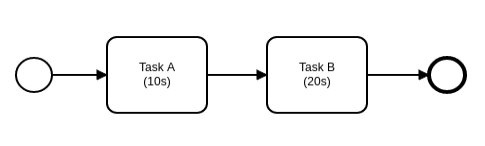
\includegraphics[width=0.5\columnwidth]{graphics/sequential-tasks}
	\caption{a process with two sequential executed tasks} 
	\label{fig:sequential-tasks} 
\end{figure}

Considering a more general process model $P$ with sequential blocks $B_1,B_2 ... B_n$ the runtime $R_P$ of process $P$ ca be calculated using the formula \ref{eq:sum-seq}. 
\begin{equation}\label{eq:sum-seq}
	R_P = \displaystyle\sum_{i=1}^{n} B_i
\end{equation}

\paragraph{Parallel Tasks}~\\
The cycle time of parallel tasks or blocks can be calculated using the maximum time of the two parallel blocks. Given the parallel block in figure \ref{fig:parallel-tasks}, this would result in a process time of 20s for this block.\cite{fundamentals}
\begin{figure}[H]
	\centering
	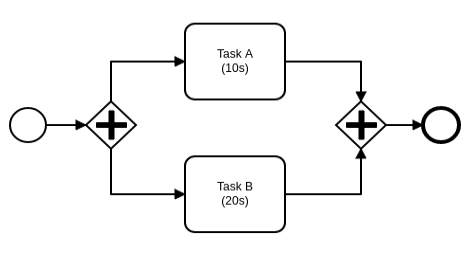
\includegraphics[width=0.5\columnwidth]{graphics/paralell-tasks}
	\caption{a process with two parallel executed tasks} 
	\label{fig:parallel-tasks} 
\end{figure}

Considering a more general process model $P$ with parallel blocks $B_1,B_2 ... B_n$ the runtime $R_P$ of process $P$ ca be calculated using the formula \ref{eq:sum-par}. 
\begin{equation}\label{eq:sum-par}
	R_P = \operatorname*{arg\,max}_i B_i
\end{equation}

\paragraph{Alternative Sequence Flows}~\\
When having two or more alternative sequence flows with different execution times, additional knowledge about the likelihood of those alternatives is needed \cite{fundamentals}. When looking at the alternative executed tasks in figure \ref{fig:alternative-tasks}, the average cycle time can be estimated by multiplying the probability of the two alternatives with the execution time of the tasks and summing up the results. This results in $10 * 70\% + 20 * 30\% = 13s$ estimated execution time. 

\begin{figure}[H]
	\centering
	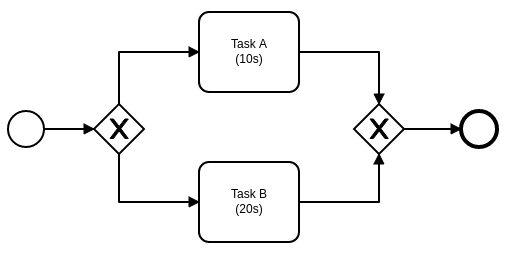
\includegraphics[width=0.5\columnwidth]{graphics/alternative-tasks}
	\caption{a process with two alternative sequence flows} 
	\label{fig:alternative-tasks} 
\end{figure}

Generally, the cycle time $R_P$ of a process $P$ with one or more alternative blocks, that have the runtimes $B_1,B_2 ... B_n$ and a likelihood of $p_1,p_2 ... p_n$ respectively, is estimated with the formula \ref{eq:alternative-seq}. \cite{fundamentals}

\begin{equation}\label{eq:alternative-seq}
	R_P = \displaystyle\sum_{i=1}^{n} B_i * p_i
\end{equation}

\paragraph{Repeating Tasks}~\\
According to the BPMN-Standard\cite{bpmnstandard} defined by OMG, there are multiple ways to indicate that a task or sequence is executed more than once: 

\begin{itemize}
	
	\item \textbf{Multiple Instances}: Three lines in the bottom of the task indicate that a task is executed multiple times - once for every instance or element. There are two kinds of multi-instance tasks: sequential, meaning the instances are processes one after another and parallel, meaning the instances are processed at the same time. 
	\begin{figure}[H]
		\centering
		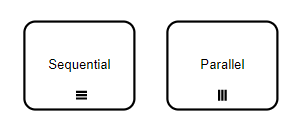
\includegraphics[width=0.4\columnwidth]{graphics/multi-instance-tasks}
		\caption{Multiple instance tasks} 
		\label{fig:muliti-instance-tasks} 
	\end{figure}
	The execution time of these tasks can be estimated using the same calculations as described above with parallel and sequential tasks.
	
	Having a process $P$ consisting of only one multi-instance task with the runtimes $B_1,B_2 ... B_n$ for each instance, the total runtime $R_P$ of process $P$ ca be calculated using the formula \ref{eq:sum-par} when the instances are executed parallel and \ref{eq:sum-seq} when the instances are executed sequential. 
	
	\item \textbf{Activity Looping}: A loop in the bottom center of the activity indicates, that this task is performed more than once. The definition on when this task repeats is specified in the \textit{loopCharacteristics}-XML Element.
	\begin{figure}[H]
		\centering
		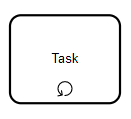
\includegraphics[width=0.2\columnwidth]{graphics/looped-task}
		\caption{A task with activity looping} 
		\label{fig:activity-looping} 
	\end{figure}
	\item \textbf{Sequence Flow Looping}: Whenever a whole sequence flow instead of a task needs to be repeated, a \textit{Sequence Flow Looping}-pattern can be used where the looping condition is defined within a exclusive gateway. The default flow points back to the start of the repeating sequence flow. 
	\begin{figure}[H]
		\centering
		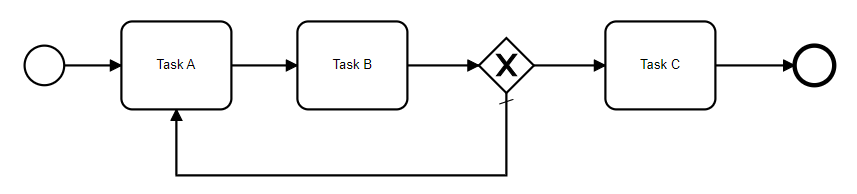
\includegraphics[width=0.9\columnwidth]{graphics/sequence-flow-looping}
		\caption{The sequence flow looping pattern} 
		\label{fig:sequence-flow-looping} 
	\end{figure}
	
	The execution time of both \textbf{sequence flow looping} sequences and \textbf{activity looping} tasks are dependent on the probability that these sequences are repeated. Looking at the two equivalent processes in \ref{fig:repeated-example} the probability of Task A repeating is 20\% for each loop taken. Task A is always executed at least once. The probability for Task A being executed twice is $20\% = 0.2$. The probability of Task A being executed three times is $0.2 * 0.2 = 0.04$. Following this pattern, the execution time can be estimated with the infinite sum $\displaystyle\sum_{i=1}^{\infty} 0.2^i * 10s$.
	
	
	\begin{figure}[H]
		\centering
		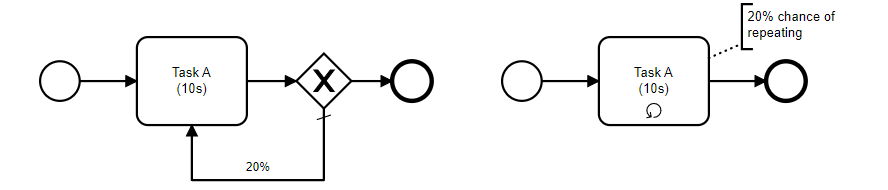
\includegraphics[width=0.9\columnwidth]{graphics/repeated-example}
		\caption{a process with sequence flow looping (left) and the equivalent using activity looping (right)} 
		\label{fig:repeated-example} 
	\end{figure}
	
	Generally the total execution time  $R_P$ of a repeated sequence where the inner part has an execution time of $R_{Repeated}$ and a probability of $p, 0 < p < 1$  to be repeated in each loop can be calculated using the formula int \ref{eq:rep-runtime}
	
	\begin{equation}\label{eq:rep-runtime}
		R_P = \displaystyle\sum_{i=1}^{\infty} p^i * R_{Repeated}
	\end{equation}
\end{itemize}


\paragraph{Queues}
%See https://link.springer.com/content/pdf/10.1007/11837862.pdf:
%An Approximate Analysis of Expected Cycle Time in Business Process Execution
As mentioned before, the \gls{cycle-time} of a process consists of the time the process is actively executed (\textit{processing time}) and the time the process spends waiting (\textit{waiting time}). In the previous section basic flow analysis was introduced to approximate and analyze these measures.  
While the processing time can be approximated using basic flow analysis, getting an idea about the total expected waiting time of a process is more complex since flow analysis as it has no tool to estimate queuing time. 

To bridge this gap, the flow analysis can be extended using a queuing approximation algorithm \cite{ha2006approximate}.


\subsection{Cycle Time Efficiency \& Littles Law}
% cite : little2008little
As mentioned before, the \gls{cycle-time} (CT) of a process consists of the time the process is actively executed (\textit{processing time}) and the time the process spends waiting (\textit{waiting time}). Besides looking at the overall cycle time, it might also be useful to analyze the processing time relative to the cycle time. This measure is called \textit{cycle time efficiency}. In this context, the \textit{processing time} is often also called \textit{theoretical cycle time (TCT)}. The \textit{cycle time efficiency} (CTE) can be calculated using the formula \ref{eq:cte}.\cite{fundamentals}

\begin{equation}\label{eq:cte}
	CTE = \dfrac{TCT}{CT}
\end{equation}

The theoretical cycle (TCT) time can be calculated by applying flow analysis. For determining the cycle time (CT) two other measures are needed. 

The first one is the \textit{arrival rate ($\lambda$)} that denotes the average number of process instances that start the process in a given period. The second measure needed is the \textit{work-in-process (WIP)} which is the average number of active process instances at any given time. If the WIP is stable, meaning it does not increase infinitely, the Process itself is called stable. Those three measures, the arrival rate $\lambda$, the WIP, and the cycle time (CT) are related through \textit{Littles Law} which is described in formula \ref{eq:littles-law}.\cite{little2008little}

\begin{equation}\label{eq:littles-law}
	WIP = \lambda * CT
\end{equation}

Usually, the actual cycle time of a process is harder to determine than the WIP or the arrival time, therefore one can transform \textit{Littles Law} to determine the cycle time using the other two measures (see formula \ref{eq:littles-law-transf}).
\begin{equation}\label{eq:littles-law-transf}
	CT = \dfrac{WIP}{\lambda}
\end{equation}